\documentclass[twoside]{book}

% Packages required by doxygen
\usepackage{fixltx2e}
\usepackage{calc}
\usepackage{doxygen}
\usepackage[export]{adjustbox} % also loads graphicx
\usepackage{graphicx}
\usepackage[utf8]{inputenc}
\usepackage{makeidx}
\usepackage{multicol}
\usepackage{multirow}
\PassOptionsToPackage{warn}{textcomp}
\usepackage{textcomp}
\usepackage[nointegrals]{wasysym}
\usepackage[table]{xcolor}

% Font selection
\usepackage[T1]{fontenc}
\usepackage[scaled=.90]{helvet}
\usepackage{courier}
\usepackage{amssymb}
\usepackage{sectsty}
\renewcommand{\familydefault}{\sfdefault}
\allsectionsfont{%
  \fontseries{bc}\selectfont%
  \color{darkgray}%
}
\renewcommand{\DoxyLabelFont}{%
  \fontseries{bc}\selectfont%
  \color{darkgray}%
}
\newcommand{\+}{\discretionary{\mbox{\scriptsize$\hookleftarrow$}}{}{}}

% Page & text layout
\usepackage{geometry}
\geometry{%
  a4paper,%
  top=2.5cm,%
  bottom=2.5cm,%
  left=2.5cm,%
  right=2.5cm%
}
\tolerance=750
\hfuzz=15pt
\hbadness=750
\setlength{\emergencystretch}{15pt}
\setlength{\parindent}{0cm}
\setlength{\parskip}{3ex plus 2ex minus 2ex}
\makeatletter
\renewcommand{\paragraph}{%
  \@startsection{paragraph}{4}{0ex}{-1.0ex}{1.0ex}{%
    \normalfont\normalsize\bfseries\SS@parafont%
  }%
}
\renewcommand{\subparagraph}{%
  \@startsection{subparagraph}{5}{0ex}{-1.0ex}{1.0ex}{%
    \normalfont\normalsize\bfseries\SS@subparafont%
  }%
}
\makeatother

% Headers & footers
\usepackage{fancyhdr}
\pagestyle{fancyplain}
\fancyhead[LE]{\fancyplain{}{\bfseries\thepage}}
\fancyhead[CE]{\fancyplain{}{}}
\fancyhead[RE]{\fancyplain{}{\bfseries\leftmark}}
\fancyhead[LO]{\fancyplain{}{\bfseries\rightmark}}
\fancyhead[CO]{\fancyplain{}{}}
\fancyhead[RO]{\fancyplain{}{\bfseries\thepage}}
\fancyfoot[LE]{\fancyplain{}{}}
\fancyfoot[CE]{\fancyplain{}{}}
\fancyfoot[RE]{\fancyplain{}{\bfseries\scriptsize Generated by Doxygen }}
\fancyfoot[LO]{\fancyplain{}{\bfseries\scriptsize Generated by Doxygen }}
\fancyfoot[CO]{\fancyplain{}{}}
\fancyfoot[RO]{\fancyplain{}{}}
\renewcommand{\footrulewidth}{0.4pt}
\renewcommand{\chaptermark}[1]{%
  \markboth{#1}{}%
}
\renewcommand{\sectionmark}[1]{%
  \markright{\thesection\ #1}%
}

% Indices & bibliography
\usepackage{natbib}
\usepackage[titles]{tocloft}
\setcounter{tocdepth}{3}
\setcounter{secnumdepth}{5}
\makeindex

% Hyperlinks (required, but should be loaded last)
\usepackage{ifpdf}
\ifpdf
  \usepackage[pdftex,pagebackref=true]{hyperref}
\else
  \usepackage[ps2pdf,pagebackref=true]{hyperref}
\fi
\hypersetup{%
  colorlinks=true,%
  linkcolor=blue,%
  citecolor=blue,%
  unicode%
}

% Custom commands
\newcommand{\clearemptydoublepage}{%
  \newpage{\pagestyle{empty}\cleardoublepage}%
}

\usepackage{caption}
\captionsetup{labelsep=space,justification=centering,font={bf},singlelinecheck=off,skip=4pt,position=top}

%===== C O N T E N T S =====

\begin{document}

% Titlepage & ToC
\hypersetup{pageanchor=false,
             bookmarksnumbered=true,
             pdfencoding=unicode
            }
\pagenumbering{roman}
\begin{titlepage}
\vspace*{7cm}
\begin{center}%
{\Large My Project }\\
\vspace*{1cm}
{\large Generated by Doxygen 1.8.11}\\
\end{center}
\end{titlepage}
\clearemptydoublepage
\tableofcontents
\clearemptydoublepage
\pagenumbering{arabic}
\hypersetup{pageanchor=true}

%--- Begin generated contents ---
\chapter{Hierarchical Index}
\section{Class Hierarchy}
This inheritance list is sorted roughly, but not completely, alphabetically\+:\begin{DoxyCompactList}
\item \contentsline{section}{Fruit}{\pageref{classFruit}}{}
\begin{DoxyCompactList}
\item \contentsline{section}{Apple}{\pageref{classApple}}{}
\item \contentsline{section}{Grape}{\pageref{classGrape}}{}
\item \contentsline{section}{Orange}{\pageref{classOrange}}{}
\end{DoxyCompactList}
\item \contentsline{section}{List}{\pageref{classList}}{}
\item \contentsline{section}{List\+:\+:Node}{\pageref{structList_1_1Node}}{}
\end{DoxyCompactList}

\chapter{Class Index}
\section{Class List}
Here are the classes, structs, unions and interfaces with brief descriptions\+:\begin{DoxyCompactList}
\item\contentsline{section}{\hyperlink{structnode}{node} }{\pageref{structnode}}{}
\item\contentsline{section}{\hyperlink{structnode1}{node1} }{\pageref{structnode1}}{}
\item\contentsline{section}{\hyperlink{structnode__info}{node\+\_\+info} }{\pageref{structnode__info}}{}
\end{DoxyCompactList}

\chapter{File Index}
\section{File List}
Here is a list of all files with brief descriptions\+:\begin{DoxyCompactList}
\item\contentsline{section}{\hyperlink{Lab1_8c}{Lab1.\+c} }{\pageref{Lab1_8c}}{}
\end{DoxyCompactList}

\chapter{Class Documentation}
\hypertarget{classB__class}{}\section{B\+\_\+class Class Reference}
\label{classB__class}\index{B\+\_\+class@{B\+\_\+class}}


Inheritance diagram for B\+\_\+class\+:
\nopagebreak
\begin{figure}[H]
\begin{center}
\leavevmode
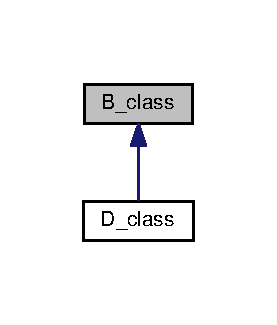
\includegraphics[width=133pt]{classB__class__inherit__graph}
\end{center}
\end{figure}
\subsection*{Public Member Functions}
\begin{DoxyCompactItemize}
\item 
void \hyperlink{classB__class_affa3773b8077feb5b2f5127c60b2079c}{put\+\_\+author} (char $\ast$s)
\item 
void \hyperlink{classB__class_a9529aa9d79a76ad2e0e4c8b4d368cb80}{show\+\_\+author} ()
\end{DoxyCompactItemize}
\subsection*{Private Attributes}
\begin{DoxyCompactItemize}
\item 
char \hyperlink{classB__class_a7e1c4f3dce456407e4cfb0ab8187a4c7}{author} \mbox{[}80\mbox{]}
\end{DoxyCompactItemize}


\subsection{Member Function Documentation}
\index{B\+\_\+class@{B\+\_\+class}!put\+\_\+author@{put\+\_\+author}}
\index{put\+\_\+author@{put\+\_\+author}!B\+\_\+class@{B\+\_\+class}}
\subsubsection[{\texorpdfstring{put\+\_\+author(char $\ast$s)}{put_author(char *s)}}]{\setlength{\rightskip}{0pt plus 5cm}void B\+\_\+class\+::put\+\_\+author (
\begin{DoxyParamCaption}
\item[{char $\ast$}]{s}
\end{DoxyParamCaption}
)\hspace{0.3cm}{\ttfamily [inline]}}\hypertarget{classB__class_affa3773b8077feb5b2f5127c60b2079c}{}\label{classB__class_affa3773b8077feb5b2f5127c60b2079c}

\begin{DoxyCode}
8 \{ strcpy(\hyperlink{classB__class_a7e1c4f3dce456407e4cfb0ab8187a4c7}{author}, s); \}
\end{DoxyCode}
\index{B\+\_\+class@{B\+\_\+class}!show\+\_\+author@{show\+\_\+author}}
\index{show\+\_\+author@{show\+\_\+author}!B\+\_\+class@{B\+\_\+class}}
\subsubsection[{\texorpdfstring{show\+\_\+author()}{show_author()}}]{\setlength{\rightskip}{0pt plus 5cm}void B\+\_\+class\+::show\+\_\+author (
\begin{DoxyParamCaption}
{}
\end{DoxyParamCaption}
)\hspace{0.3cm}{\ttfamily [inline]}}\hypertarget{classB__class_a9529aa9d79a76ad2e0e4c8b4d368cb80}{}\label{classB__class_a9529aa9d79a76ad2e0e4c8b4d368cb80}

\begin{DoxyCode}
9 \{ cout << \hyperlink{classB__class_a7e1c4f3dce456407e4cfb0ab8187a4c7}{author} << \textcolor{stringliteral}{"\(\backslash\)n"}; \}
\end{DoxyCode}


\subsection{Member Data Documentation}
\index{B\+\_\+class@{B\+\_\+class}!author@{author}}
\index{author@{author}!B\+\_\+class@{B\+\_\+class}}
\subsubsection[{\texorpdfstring{author}{author}}]{\setlength{\rightskip}{0pt plus 5cm}char B\+\_\+class\+::author\mbox{[}80\mbox{]}\hspace{0.3cm}{\ttfamily [private]}}\hypertarget{classB__class_a7e1c4f3dce456407e4cfb0ab8187a4c7}{}\label{classB__class_a7e1c4f3dce456407e4cfb0ab8187a4c7}


The documentation for this class was generated from the following file\+:\begin{DoxyCompactItemize}
\item 
\hyperlink{Polymorphism_8cpp}{Polymorphism.\+cpp}\end{DoxyCompactItemize}

\hypertarget{classD__class}{}\section{D\+\_\+class Class Reference}
\label{classD__class}\index{D\+\_\+class@{D\+\_\+class}}


Inheritance diagram for D\+\_\+class\+:
\nopagebreak
\begin{figure}[H]
\begin{center}
\leavevmode
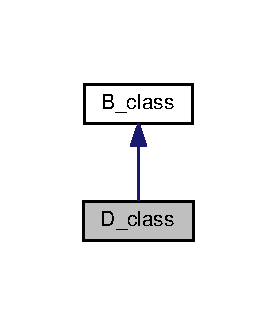
\includegraphics[width=133pt]{classD__class__inherit__graph}
\end{center}
\end{figure}


Collaboration diagram for D\+\_\+class\+:
\nopagebreak
\begin{figure}[H]
\begin{center}
\leavevmode
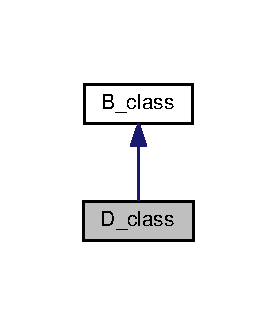
\includegraphics[width=133pt]{classD__class__coll__graph}
\end{center}
\end{figure}
\subsection*{Public Member Functions}
\begin{DoxyCompactItemize}
\item 
void \hyperlink{classD__class_aa7f2a7577198caa052f7022e26f2c06b}{put\+\_\+title} (char $\ast$num)
\item 
void \hyperlink{classD__class_af2d261ea960afdefaabf2af43c63e257}{show\+\_\+title} ()
\end{DoxyCompactItemize}
\subsection*{Private Attributes}
\begin{DoxyCompactItemize}
\item 
char \hyperlink{classD__class_a0b934cdee41ce168d60d496ea0135025}{title} \mbox{[}80\mbox{]}
\end{DoxyCompactItemize}


\subsection{Member Function Documentation}
\index{D\+\_\+class@{D\+\_\+class}!put\+\_\+title@{put\+\_\+title}}
\index{put\+\_\+title@{put\+\_\+title}!D\+\_\+class@{D\+\_\+class}}
\subsubsection[{\texorpdfstring{put\+\_\+title(char $\ast$num)}{put_title(char *num)}}]{\setlength{\rightskip}{0pt plus 5cm}void D\+\_\+class\+::put\+\_\+title (
\begin{DoxyParamCaption}
\item[{char $\ast$}]{num}
\end{DoxyParamCaption}
)\hspace{0.3cm}{\ttfamily [inline]}}\hypertarget{classD__class_aa7f2a7577198caa052f7022e26f2c06b}{}\label{classD__class_aa7f2a7577198caa052f7022e26f2c06b}

\begin{DoxyCode}
15                             \{
16     strcpy(\hyperlink{classD__class_a0b934cdee41ce168d60d496ea0135025}{title}, num);
17   \}
\end{DoxyCode}
\index{D\+\_\+class@{D\+\_\+class}!show\+\_\+title@{show\+\_\+title}}
\index{show\+\_\+title@{show\+\_\+title}!D\+\_\+class@{D\+\_\+class}}
\subsubsection[{\texorpdfstring{show\+\_\+title()}{show_title()}}]{\setlength{\rightskip}{0pt plus 5cm}void D\+\_\+class\+::show\+\_\+title (
\begin{DoxyParamCaption}
{}
\end{DoxyParamCaption}
)\hspace{0.3cm}{\ttfamily [inline]}}\hypertarget{classD__class_af2d261ea960afdefaabf2af43c63e257}{}\label{classD__class_af2d261ea960afdefaabf2af43c63e257}

\begin{DoxyCode}
18                     \{
19     cout << \textcolor{stringliteral}{"Title: "};
20     cout <<  \hyperlink{classD__class_a0b934cdee41ce168d60d496ea0135025}{title} << \textcolor{stringliteral}{"\(\backslash\)n"};
21   \}
\end{DoxyCode}


\subsection{Member Data Documentation}
\index{D\+\_\+class@{D\+\_\+class}!title@{title}}
\index{title@{title}!D\+\_\+class@{D\+\_\+class}}
\subsubsection[{\texorpdfstring{title}{title}}]{\setlength{\rightskip}{0pt plus 5cm}char D\+\_\+class\+::title\mbox{[}80\mbox{]}\hspace{0.3cm}{\ttfamily [private]}}\hypertarget{classD__class_a0b934cdee41ce168d60d496ea0135025}{}\label{classD__class_a0b934cdee41ce168d60d496ea0135025}


The documentation for this class was generated from the following file\+:\begin{DoxyCompactItemize}
\item 
\hyperlink{Polymorphism_8cpp}{Polymorphism.\+cpp}\end{DoxyCompactItemize}

\chapter{File Documentation}
\hypertarget{Polymorphism_8cpp}{}\section{Polymorphism.\+cpp File Reference}
\label{Polymorphism_8cpp}\index{Polymorphism.\+cpp@{Polymorphism.\+cpp}}
{\ttfamily \#include $<$iostream$>$}\\*
{\ttfamily \#include $<$cstring$>$}\\*
Include dependency graph for Polymorphism.\+cpp\+:
\nopagebreak
\begin{figure}[H]
\begin{center}
\leavevmode
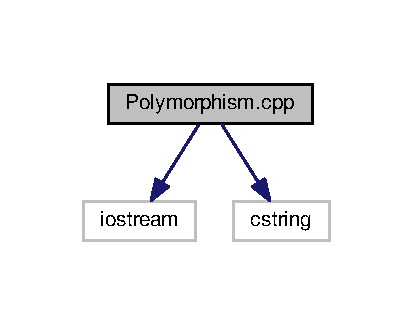
\includegraphics[width=198pt]{Polymorphism_8cpp__incl}
\end{center}
\end{figure}
\subsection*{Classes}
\begin{DoxyCompactItemize}
\item 
class \hyperlink{classB__class}{B\+\_\+class}
\item 
class \hyperlink{classD__class}{D\+\_\+class}
\end{DoxyCompactItemize}
\subsection*{Functions}
\begin{DoxyCompactItemize}
\item 
int \hyperlink{Polymorphism_8cpp_ae66f6b31b5ad750f1fe042a706a4e3d4}{main} ()
\end{DoxyCompactItemize}


\subsection{Function Documentation}
\index{Polymorphism.\+cpp@{Polymorphism.\+cpp}!main@{main}}
\index{main@{main}!Polymorphism.\+cpp@{Polymorphism.\+cpp}}
\subsubsection[{\texorpdfstring{main()}{main()}}]{\setlength{\rightskip}{0pt plus 5cm}int main (
\begin{DoxyParamCaption}
{}
\end{DoxyParamCaption}
)}\hypertarget{Polymorphism_8cpp_ae66f6b31b5ad750f1fe042a706a4e3d4}{}\label{Polymorphism_8cpp_ae66f6b31b5ad750f1fe042a706a4e3d4}

\begin{DoxyCode}
25 \{
26   \hyperlink{classB__class}{B\_class} *p;
27   \hyperlink{classB__class}{B\_class} B\_ob;
28 
29   \hyperlink{classD__class}{D\_class} *dp;
30   \hyperlink{classD__class}{D\_class} D\_ob;
31 
32   p = &B\_ob;  \textcolor{comment}{// address of base}
33 
34   \textcolor{comment}{// Access B\_class via pointer.}
35   p->\hyperlink{classB__class_affa3773b8077feb5b2f5127c60b2079c}{put\_author}(\textcolor{stringliteral}{"Tom Clancy"});
36 
37   \textcolor{comment}{// Access D\_class via base pointer.}
38   p = &D\_ob;
39   p->\hyperlink{classB__class_affa3773b8077feb5b2f5127c60b2079c}{put\_author}(\textcolor{stringliteral}{"William Shakespeare"});
40 
41   \textcolor{comment}{// Show that each author went into proper object.}
42   B\_ob.\hyperlink{classB__class_a9529aa9d79a76ad2e0e4c8b4d368cb80}{show\_author}();
43   D\_ob.\hyperlink{classB__class_a9529aa9d79a76ad2e0e4c8b4d368cb80}{show\_author}();
44   cout << \textcolor{stringliteral}{"\(\backslash\)n"};
45 
46   \textcolor{comment}{/* Since put\_title() and show\_title() are not part}
47 \textcolor{comment}{     of the base class, they are not accessible via}
48 \textcolor{comment}{     the base pointer p and must be accessed either}
49 \textcolor{comment}{     directly, or, as shown here, through a pointer to the}
50 \textcolor{comment}{     derived type.}
51 \textcolor{comment}{  */}
52   dp = &D\_ob;
53   dp->\hyperlink{classD__class_aa7f2a7577198caa052f7022e26f2c06b}{put\_title}(\textcolor{stringliteral}{"The Tempest"});
54   p->\hyperlink{classB__class_a9529aa9d79a76ad2e0e4c8b4d368cb80}{show\_author}(); \textcolor{comment}{// either p or dp can be used here.}
55   dp->\hyperlink{classD__class_af2d261ea960afdefaabf2af43c63e257}{show\_title}( );
56 
57   \textcolor{keywordflow}{return} 0;
58 \}\end{DoxyCode}


Here is the call graph for this function\+:
\nopagebreak
\begin{figure}[H]
\begin{center}
\leavevmode
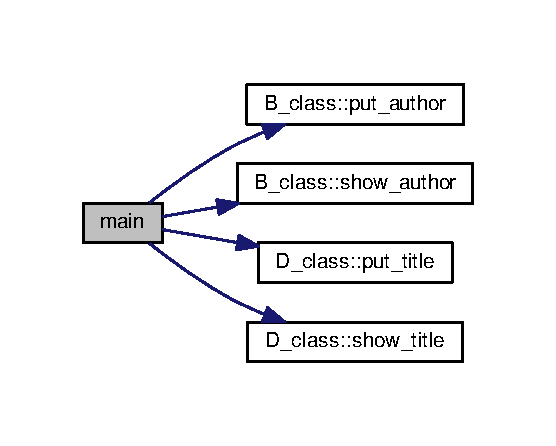
\includegraphics[width=267pt]{Polymorphism_8cpp_ae66f6b31b5ad750f1fe042a706a4e3d4_cgraph}
\end{center}
\end{figure}



%--- End generated contents ---

% Index
\backmatter
\newpage
\phantomsection
\clearemptydoublepage
\addcontentsline{toc}{chapter}{Index}
\printindex

\end{document}
